%% LyX 2.2.4 created this file.  For more info, see http://www.lyx.org/.
%% Do not edit unless you really know what you are doing.
\documentclass[english,10pt,t,aspectratio=169]{beamer}
\usepackage[T1]{fontenc}
\usepackage[latin9]{inputenc}
\setcounter{secnumdepth}{3}
\setcounter{tocdepth}{3}
\usepackage{graphicx}

\makeatletter
%%%%%%%%%%%%%%%%%%%%%%%%%%%%%% Textclass specific LaTeX commands.
 % this default might be overridden by plain title style
 \newcommand\makebeamertitle{\frame{\maketitle}}%
 % (ERT) argument for the TOC
 \AtBeginDocument{%
   \let\origtableofcontents=\tableofcontents
   \def\tableofcontents{\@ifnextchar[{\origtableofcontents}{\gobbletableofcontents}}
   \def\gobbletableofcontents#1{\origtableofcontents}
 }

%%%%%%%%%%%%%%%%%%%%%%%%%%%%%% User specified LaTeX commands.
\usepackage{upgreek}
\usetheme{desynew}
\setbeamertemplate{title graphic}[empty]
\setbeamertemplate{second logo in title page}[desycms]

\title{Presentation Title}
\subtitle{Presentation Subtitle}
\author[N. Surname]{Name Surname}
\institute[ShortConf]{Conference Name}
\date[February 22, 2022]{February 22, 2022}

\makeatother

\usepackage{babel}
\usepackage{listings}
\lstset{language=Python,
breaklines=true,
basicstyle={\ttfamily},
stringstyle={\color{brown}},
basicstyle={\tiny}}
\begin{document}
\maketitle

\begin{frame}{Fancy Slide}


\framesubtitle{Frame subtitle}

Some explanation\vspace{-0.03\paperheight}

\begin{columns}

\column{0.47\columnwidth}
\begin{center}
Title of left figure\vspace{-0.03\paperheight}
\par\end{center}

\begin{center}
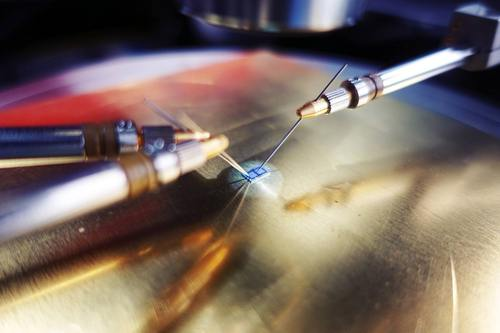
\includegraphics[width=1\columnwidth]{graphics/example_image}
\par\end{center}

\column{0.47\columnwidth}
\begin{center}
Title of right figure\vspace{-0.03\paperheight}
\par\end{center}

\begin{center}
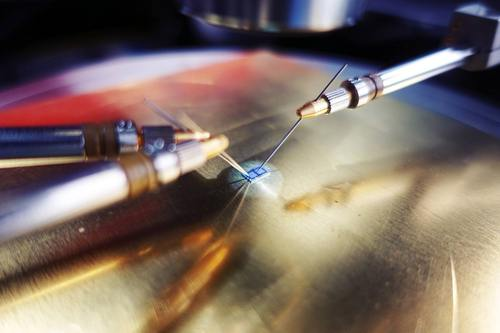
\includegraphics[width=1\columnwidth]{graphics/example_image}
\par\end{center}
\end{columns}

\begin{itemize}
\item This thing
\item That thing
\end{itemize}
\end{frame}
%
\begin{frame}{}

\begin{textblock*}{0.912\paperwidth}
(0.044\paperwidth,0.086\paperheight)
    \usebeamerfont{main title in title page}\usebeamercolor[fg]{main title on empty}%
    Thank you
\end{textblock*}%
\end{frame}

\end{document}
